\documentclass{standalone}
\usepackage{tikz}
\usetikzlibrary{shapes}

\begin{document}

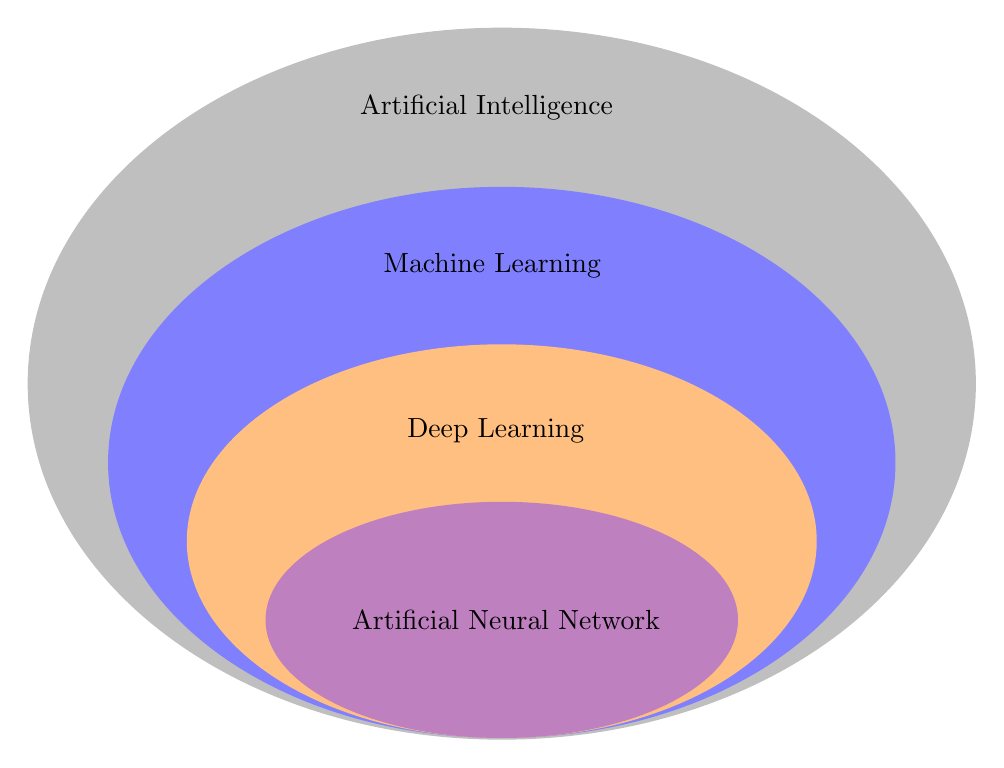
\begin{tikzpicture}[
first/.style={ellipse, minimum width=12cm, minimum height=9cm, align=center, draw=gray!50, fill=gray!50, very thick},
second/.style={ellipse, minimum width=10cm, minimum height=7cm, align=center,color=blue!50, fill=blue!50, very thick},
third/.style={ellipse, minimum width=8cm, minimum height=5cm, align=center,color=orange!50, fill=orange!50, very thick},
fourth/.style={ellipse, minimum width=6cm, minimum height=3cm,color=violet!50, fill=violet!50, very thick},
]


\node (AI) [first] at (1,0) {};
\node (ML) [second] at (1,-1) {};
\node (DL) [third] at (1,-2) {};
\node (ANN) [fourth] at (1,-3) {};
\node (a) [text width=7cm] at (2.7,3.5) {Artificial Intelligence};
\node (b) [text width=5cm] at (2,1.5) {Machine Learning};
\node (c) [text width=5cm] at (2.3,-0.6) {Deep Learning};
\node (d) [text width=5cm] at (1.6,-3) {Artificial Neural Network};

\end{tikzpicture}  
\end{document}